%%%%%%%%%%%%%%%%%%%%%%%%%%%%%%%%%%%%%%%%%%%%%%%%%%%%%%%%%%%%%%%%%%%%%%%%%%%%%%%%
%Tutorial slides on Python.
%
% Author: Prabhu Ramachandran <prabhu at aero.iitb.ac.in>
% Copyright (c) 2005-2009, Prabhu Ramachandran
%%%%%%%%%%%%%%%%%%%%%%%%%%%%%%%%%%%%%%%%%%%%%%%%%%%%%%%%%%%%%%%%%%%%%%%%%%%%%%%%

\documentclass[14pt,compress]{beamer}
%\documentclass[draft]{beamer}
%\documentclass[compress,handout]{beamer}
%\usepackage{pgfpages} 
%\pgfpagesuselayout{2 on 1}[a4paper,border shrink=5mm]

% Modified from: generic-ornate-15min-45min.de.tex
\mode<presentation>
{
  \usetheme{Warsaw}
  \useoutertheme{infolines}
  \setbeamercovered{transparent}
}

\usepackage[english]{babel}
\usepackage[latin1]{inputenc}
%\usepackage{times}
\usepackage[T1]{fontenc}

% Taken from Fernando's slides.
\usepackage{ae,aecompl}
\usepackage{mathpazo,courier,euler}
\usepackage[scaled=.95]{helvet}

\definecolor{darkgreen}{rgb}{0,0.5,0}

\usepackage{listings}
\lstset{language=Python,
    basicstyle=\ttfamily\bfseries,
    commentstyle=\color{red}\itshape,
  stringstyle=\color{darkgreen},
  showstringspaces=false,
  keywordstyle=\color{blue}\bfseries}

%%%%%%%%%%%%%%%%%%%%%%%%%%%%%%%%%%%%%%%%%%%%%%%%%%%%%%%%%%%%%%%%%%%%%%
% Macros
\setbeamercolor{emphbar}{bg=blue!20, fg=black}
\newcommand{\emphbar}[1]
{\begin{beamercolorbox}[rounded=true]{emphbar} 
      {#1}
 \end{beamercolorbox}
}
\newcounter{time}
\setcounter{time}{0}
\newcommand{\inctime}[1]{\addtocounter{time}{#1}{\tiny \thetime\ m}}

\newcommand{\typ}[1]{\texttt{#1}}

\newcommand{\kwrd}[1]{ \texttt{\textbf{\color{blue}{#1}}}  }

%%% This is from Fernando's setup.
% \usepackage{color}
% \definecolor{orange}{cmyk}{0,0.4,0.8,0.2}
% % Use and configure listings package for nicely formatted code
% \usepackage{listings}
% \lstset{
%    language=Python,
%    basicstyle=\small\ttfamily,
%    commentstyle=\ttfamily\color{blue},
%    stringstyle=\ttfamily\color{orange},
%    showstringspaces=false,
%    breaklines=true,
%    postbreak = \space\dots
% }


%%%%%%%%%%%%%%%%%%%%%%%%%%%%%%%%%%%%%%%%%%%%%%%%%%%%%%%%%%%%%%%%%%%%%%
% Title page
\title[Exercises]{Exercises}

\author[FOSSEE] {FOSSEE}

\institute[IIT Bombay] {Department of Aerospace Engineering\\IIT Bombay}
\date[] {8 November, 2009\\Day 2, Session 5}
%%%%%%%%%%%%%%%%%%%%%%%%%%%%%%%%%%%%%%%%%%%%%%%%%%%%%%%%%%%%%%%%%%%%%%

%\pgfdeclareimage[height=0.75cm]{iitmlogo}{iitmlogo}
%\logo{\pgfuseimage{iitmlogo}}


%% Delete this, if you do not want the table of contents to pop up at
%% the beginning of each subsection:
\AtBeginSubsection[]
{
  \begin{frame}<beamer>
    \frametitle{Outline}
    \tableofcontents[currentsection,currentsubsection]
  \end{frame}
}


% If you wish to uncover everything in a step-wise fashion, uncomment
% the following command: 
%\beamerdefaultoverlayspecification{<+->}

%\includeonlyframes{current,current1,current2,current3,current4,current5,current6}

%%%%%%%%%%%%%%%%%%%%%%%%%%%%%%%%%%%%%%%%%%%%%%%%%%%%%%%%%%%%%%%%%%%%%%
% DOCUMENT STARTS
\begin{document}

\begin{frame}
  \titlepage
\end{frame}

\begin{frame}{Problem 1.1}
  The aliquot of a number is defined as: the sum of the \emph{proper} divisors of the number. \\For example: 
\center{aliquot(12) = 1 + 2 + 3 + 4 + 6 = 16.}\\
  Write a function that returns the aliquot number of a given number. 
\end{frame}

\begin{frame}{Problem 1.2}
  Pair of numbers (a, b) is said to be \alert{amicable} if aliquot number of a is b and aliquot number of b is a.\\
  Example: \texttt{220, 284}\\
  Write a program that prints all four digit amicable pairs.
  
\inctime{20}
\end{frame}

%% \begin{frame}{Problem 2}
%%   Given an empty chessboard and one Bishop placed in any s%quare, say (r, c), generate the list of all squares the Bi%shop could move to.

%% \end{frame}

\begin{frame}[fragile]
  \frametitle{Problem Set 2}
  Given a string like, ``1, 3-7, 12, 15, 18-21'', produce the list \\
  \begin{lstlisting}
    [1,3,4,5,6,7,12,15,18,19,20,21]
  \end{lstlisting}
\inctime{10}
\end{frame}

\begin{frame} 
  \frametitle{Problem Set 3}
  \begin{description}
    \item[3.1] Count word frequencies in a file.
\end{description}
\inctime{5}
\end{frame}

\begin{frame}[fragile]
  \frametitle{Problem set 4}
  Central difference
  \begin{equation*}
  \frac{sin(x+h)-sin(x-h)}{2h}
  \end{equation*}
  \begin{lstlisting}
  In []: x = linspace(0, 2*pi, 100)
  In []: y = sin(x)
  In []: deltax = x[1] - x[0]
  \end{lstlisting}
  \pause
    \begin{enumerate}
      \item Given this, get the finite difference of sin in the range 0 to 2*pi
    \end{enumerate}
\end{frame}

\begin{frame}
  \frametitle{Problem Set 5}
  \begin{itemize}
      \item[5.1] Write a function that plots any regular n-gon given \typ{n}.
      \item[5.2] Consider the logistic map, $f(x) = kx(1-x)$, plot it for
          $k=2.5, 3.5$ and $4$ in the same plot.
\end{itemize}
\end{frame}

\begin{frame}[fragile] 
\frametitle{Problem Set 5}
  \begin{columns}
    \column{0.6\textwidth}
    \small{
    \begin{itemize}
      \item[3] Consider the iteration $x_{n+1} = f(x_n)$ where $f(x) = kx(1-x)$.  Plot the successive iterates of this process as explained below. 
    \end{itemize}}
    \column{0.35\textwidth}
    \hspace*{-0.5in}
  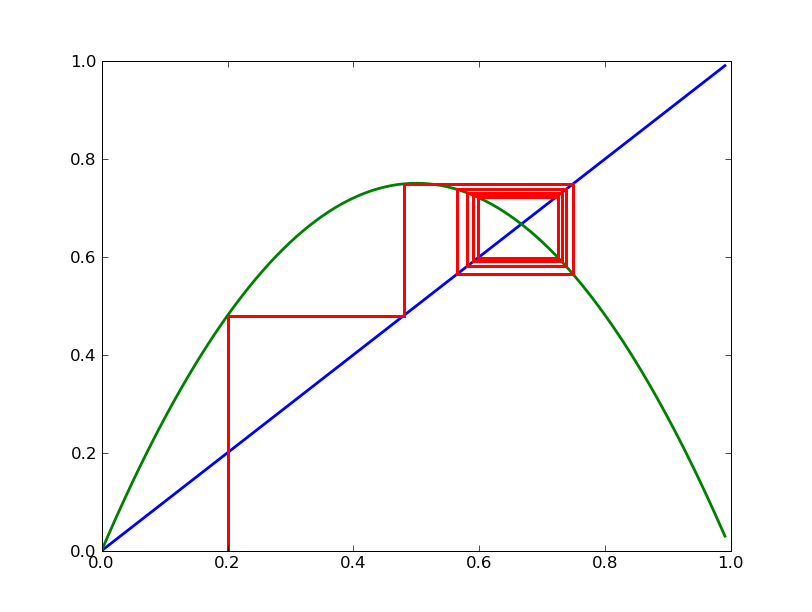
\includegraphics[height=1.6in, interpolate=true]{data/cobweb}  
\end{columns}
\end{frame}

\begin{frame}
  \frametitle{Problem Set 5.3}
  Plot the cobweb plot as follows:
  \begin{enumerate}
    \item Start at $(x_0, 0)$ ($\implies$ i=0)
    \item Draw a line to $(x_i, f(x_i))$
    \item Set $x_{i+1} = f(x_i)$
    \item Draw a line to $(x_{i+1}, x_{i+1})$
    \item $(i\implies i+1)$ 
    \item Repeat from 2 for as long as you want 
  \end{enumerate}
\inctime{20}
\end{frame}

\end{document}
